One Dimensional Systems are basically those in equation (\ref{eq:gode}) with $n=1$.
That is 
\begin{equation}{\label{eq:1d}}
  \dot{x}=f(x)
\end{equation} 
Let's start with linear systems.\\
Simplest dynamical system is given by 
\begin{equation}{\label{eq:cons}}
  \dot{x}=0 \quad \rightarrow \quad x=c 
\end{equation}
It means nothing happens with time, it's constant.
However, as we shall see, equation (\ref{eq:cons}) is extremely useful to gain insight into the dynamical structure of non-linear systems, as it is the condition for so-called {\textbf{steady states}} or {\textbf{fixed points}}.\\
Next is an equation of continous growth (or exponential growth), where change $\dot{x}$ is proportional to $x$.
\begin{equation}{\label{eq:lin1}}
  \dot{x}=\lambda x \quad \rightarrow \quad \int \frac{dx}{x} = \int \lambda \mathop{dt} \quad \rightarrow\quad x(t)= ce^{\lambda t}
\end{equation} 
As seen in Figure (\ref{fig:lin1}) the linear differential equation of continuous growth is easy to solve and its solutions are exponentially increasing, exponentially decaying or simply constant depending on the parameter $\lambda$.
\begin{figure}[h!]
  \centering
  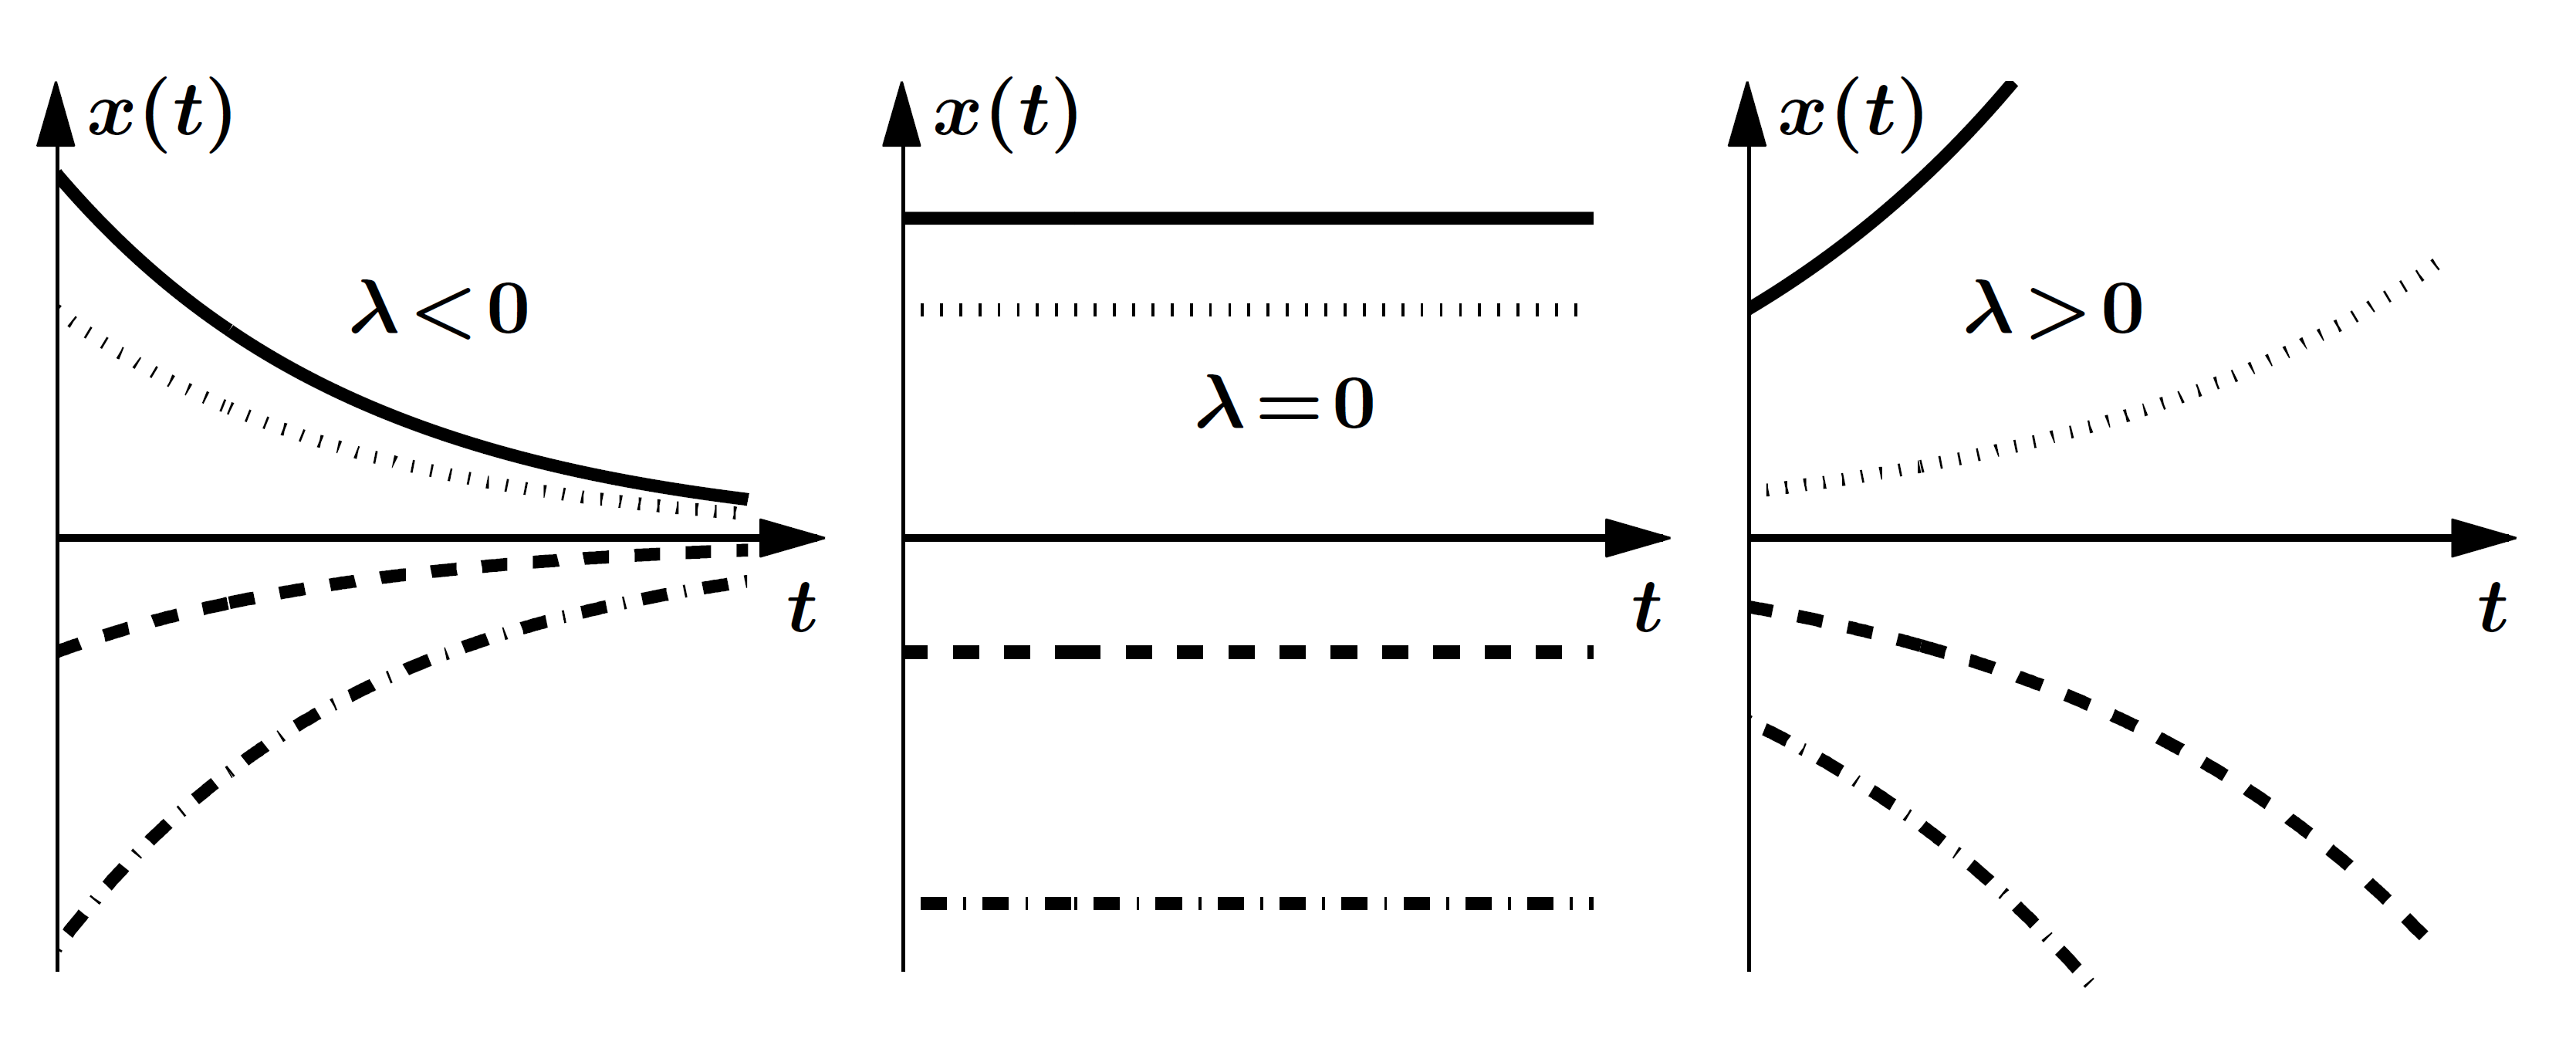
\includegraphics[width=0.5\linewidth]{lin1.png}
  \caption{Solutions $x(t)$ for the equation (\ref{eq:lin1}) for different values of $c$ (solid, dashed, dotted and dash-dotted).}
  \label{fig:lin1}
\end{figure}
If we plot $\dot{x}$ as a function of $x$, we get a {\textbf{phase space}} plot.
The graphs are straight lines given by $\dot{x}=\lambda x$ with a negative, vanishing and positive slope, respectively.
Phase space is one of most important topics in nonlinear dynamics.
\begin{figure}[h!]
  \centering
  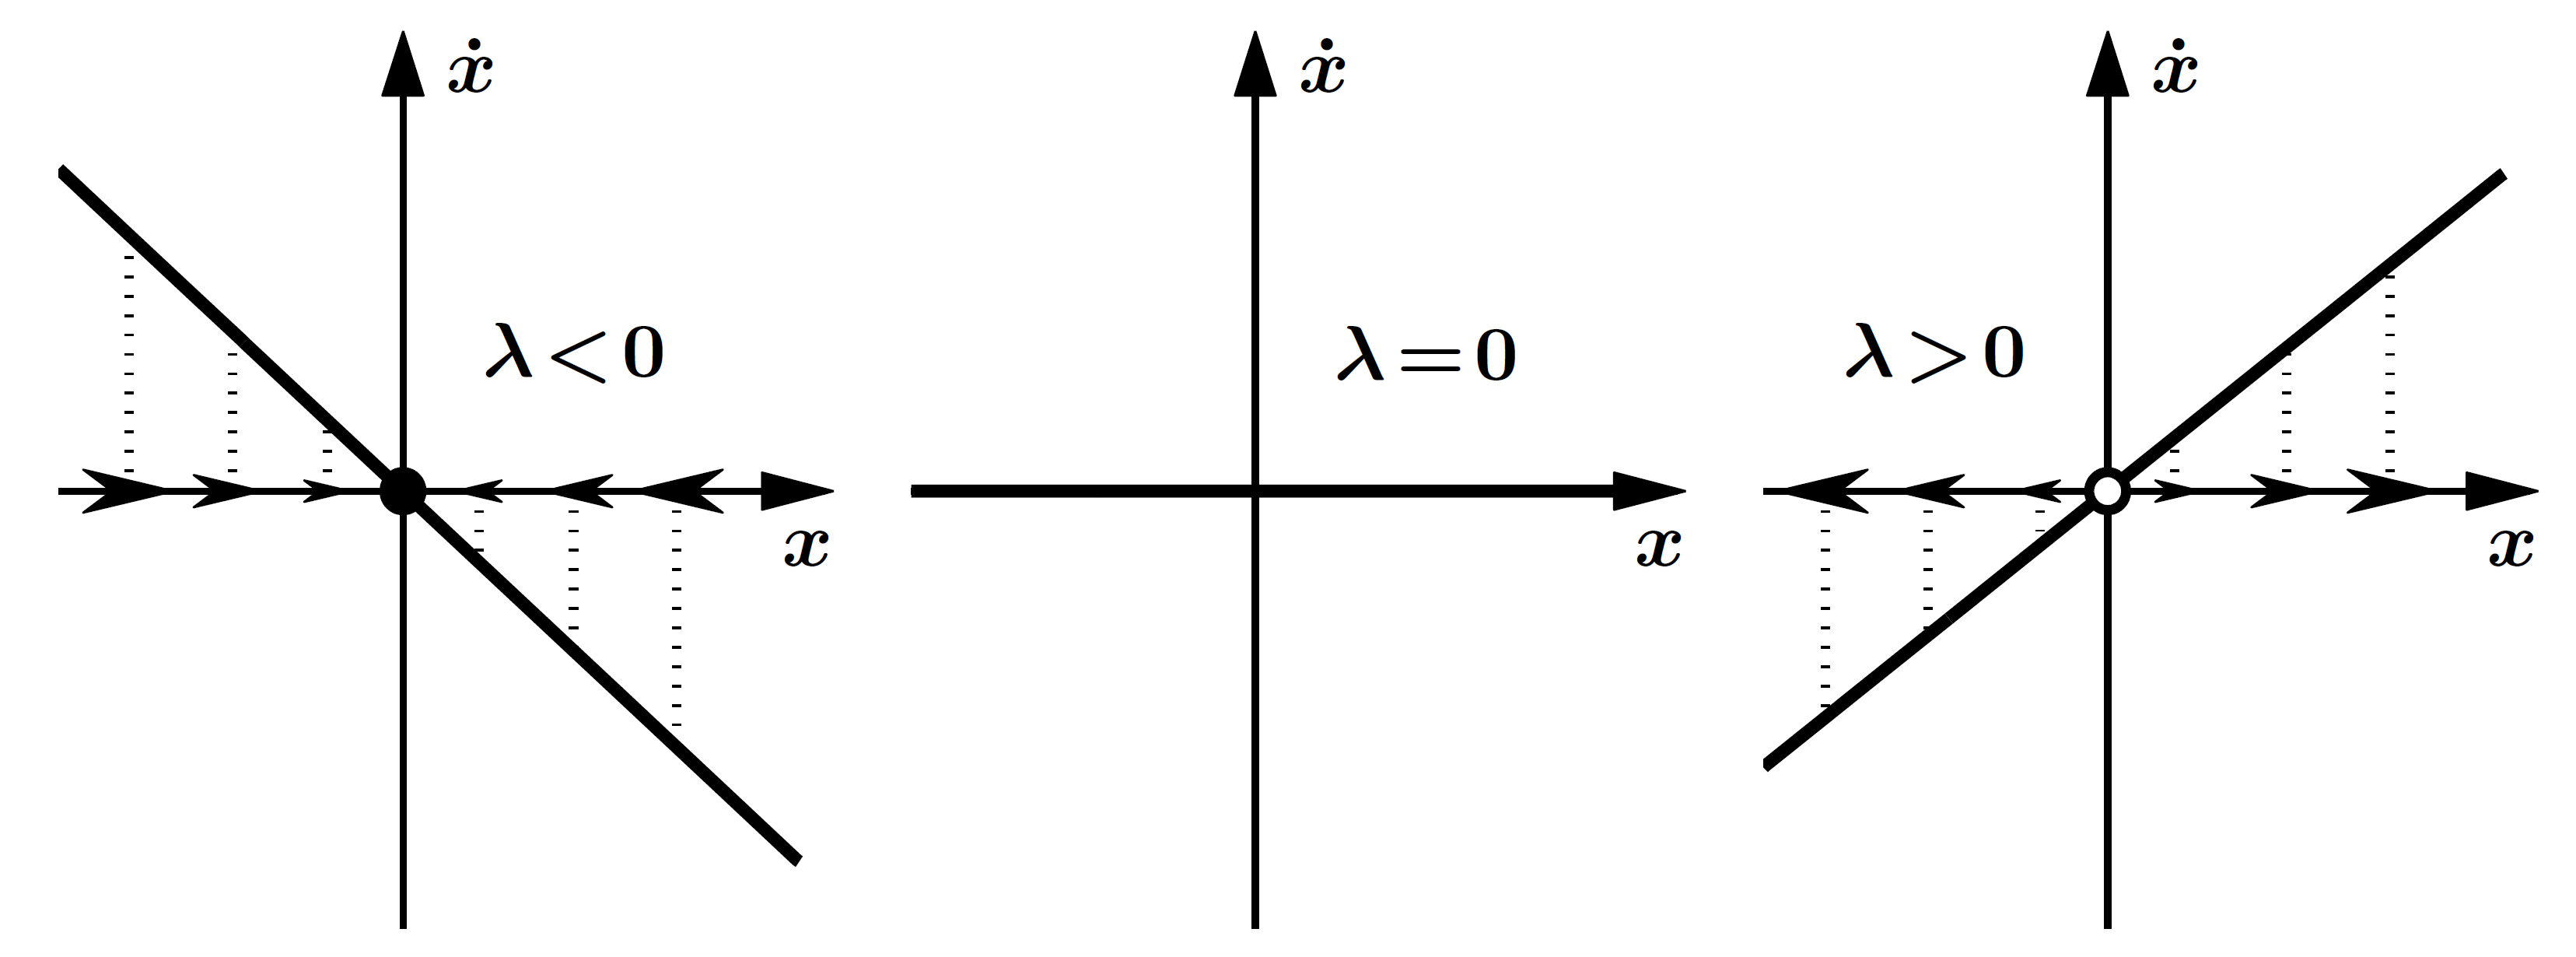
\includegraphics[width=0.5\linewidth]{bps1.png}
  \caption{Phase space plots, $\dot{x}$ as a function of $x$, for the equation (\ref{eq:lin1}).}
  \label{fig:bps1}
\end{figure}
\subsection{Flows on the Line}
Nonlinear Systems are harder to solve analytically, it's even impossible for many cases.
So, we use geometrical approach which gives qualitative behaviour of the system.
Imagine that a fluid is flowing along the real line with a local velocity $f(x)$.
This imaginary fluid is called the {\textbf{phase fluid}}, and the real line is the {\textbf{phase space}}.
The flow is to the right where $f(x)>0$ and to the left where $f(x)<0$.
\emph{Fixed points} have $f(x)=0$.
\begin{figure}[H]
  \centering
  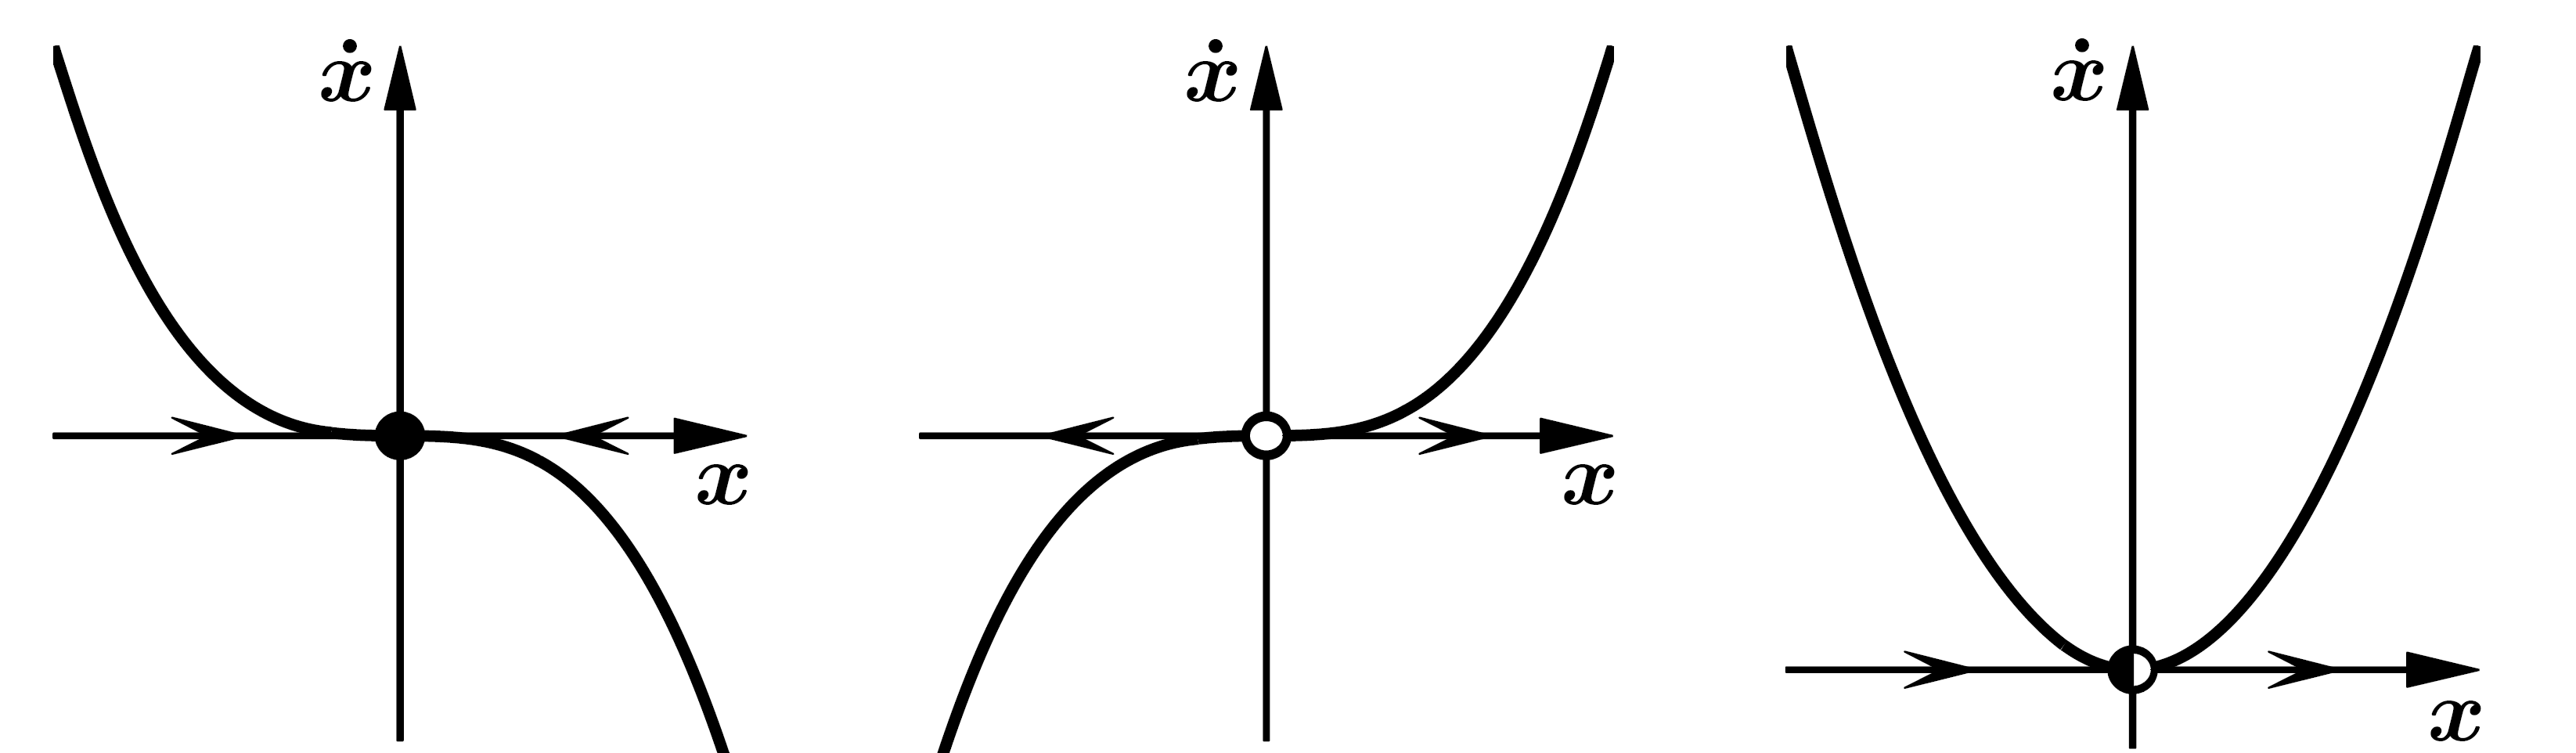
\includegraphics[width=0.5\linewidth]{bfps.png}
  \caption{Phase portrait, solid black dot(left) is a {\textbf{stable}} fixed point (the local flow is toward it) and the open dot(middle) is an {\textbf{unstable}} fixed point (the flow is away from it) and the right one is {\textbf{half-stable}} (the flow is towards it on left and away on right).}
  \label{fig:bfps}
\end{figure}
\subsection{Linear Stability Analysis}
Consider a dynamical system of the form $\dot{x}=f(x)$ and the Taylor expansion around one of its fixed points $\tilde{x}$ and let $\xi=x-\tilde{x}$, then $\dot{\xi}=\dot{x}$
\begin{equation}{\label{eq:lsa1}}
  \dot{x}=f(x) \approx \underbrace{f(\tilde{x})}_{=0}+f^\prime(\tilde{x})\underbrace{(x-\tilde{x})}_{=\xi}+\frac{1}{2!}f^{\prime \prime}(\tilde{x})\underbrace{(x-\tilde{x})^2}_{=\xi^2}+\cdots
\end{equation}
$f(\tilde{x})$ vanishes as it is a fixed point, $|\xi|$ is small as we assume $x$ to be in the vicinity of $\tilde{x}$, and therefore $\xi^2$ is tiny and can be neglected.
Taken together, we obtain an approximation of (\ref{eq:lsa1}) around the fixed point $\tilde{x}$.
\begin{equation}{\label{eq:lsa2}}
  \dot{\xi} = f^\prime(\tilde{x})\ \xi = \lambda\ \xi
\end{equation}
Now, equation (\ref{eq:lsa2}) is similar to equation (\ref{eq:lin1}).
The slope $f^\prime(\tilde{x})$ at the fixed point determines its stability\footnote{Our analysis fails for some $f(x)$ in case where solution is not unique or does not exist, See Theorem (\ref{thm:eut}).}, if $f^\prime(\tilde{x})>0$ then $\tilde{x}$ is a \emph{unstable fixed point} and if $f^\prime(\tilde{x})<0$ then $\tilde{x}$ is a \emph{stable fixed point}.
$1/f^\prime(\tilde{x})$ is a {\textbf{characteristic time scale}}, it determines the time required for $x(t)$ to vary significantly in the neighborhood of $\tilde{x}$.
\subsection{Potential Functions}{\label{sec:pf}}
A second way of representing the dynamics of such systems graphically is the landscape defined by its \emph{potential function}.
The potential of a dynamical system is a function $V(x)$ such that the relation
\begin{equation}
  \dot{x}=f(x)= -\frac{dV(x)}{dx}
\end{equation}
is fulfilled.
All one-dimensional systems have a potential function.\\
As time evolves, either the value of the potential function decreases, or it stays constant if a local or global minimum of $V(x)$ has been reached.
This behavior can easily be seen by calculating the derivative of $V$ with respect to time
\begin{equation}
  \dot{V}=\frac{dV(x)}{dt}=\underbrace{\frac{dV}{dx}}_{-\dot{x}}\underbrace{\frac{dx}{dt}}_{\dot{x}}=-\left\{\frac{dV}{dx}\right\}^2=-\dot{x}^2\leq0
\end{equation}
Local \emph{minima} of $V$ correspond to {\textbf{stable}} fixed points, local \emph{maxima} correspond to {\textbf{unstable}} fixed points, {\textbf{half-stable}} fixed points are found at locations where the tangent at an \emph{inflection point} is horizontal.
\subsubsection{Impossibility of Oscillations}
Fixed points dominate the dynamics of first-order systems.
Trajectories either approach a fixed point, or diverged to $\pm\infty$.
The reason is that trajectories are forced to increase or decrease monotonically, or remain constant.
If a fixed point is regarded as an equilibrium solution, the approach to equilibrium is always monotonic-overshoot and damped oscillations can never occur in a first-order system.
Hence there are no periodic solutions to $\dot{x}=f(x)$.
\subsection{Flows on the Circle}
Periodic systems can be realized in one dimension with dynamics that take place not on a line but on a circle.
The state variable here is not $x$, it is $\theta$ with $0\leq\theta<2\pi$ or $-\pi\leq\theta<\pi$.
The general form here is
\begin{equation}
  \dot{\theta}=f(\theta)\ \text{with}\ f(\theta+2\pi)=f(\theta)
\end{equation}
The function $f(\pi)$ has to be $2\pi-$periodic to ensure that it has the same value at $\theta=0$ and $\theta=2\pi$, which are the same points.
\subsubsection{Nonuniform Oscillator}{\label{sec:nuo}}
It has the equation
\begin{equation}
  \dot{\theta}=\omega-a\sin\theta
\end{equation}
The parameter $a$ introduces a nonuniformity in the flow around the circle, the flow is fastest at $\theta=-\pi/2$ and slowest at $\theta=\pi/2$.
\begin{figure}[H]
  \centering
  \begin{subfigure}{0.45\linewidth}
    \centering
    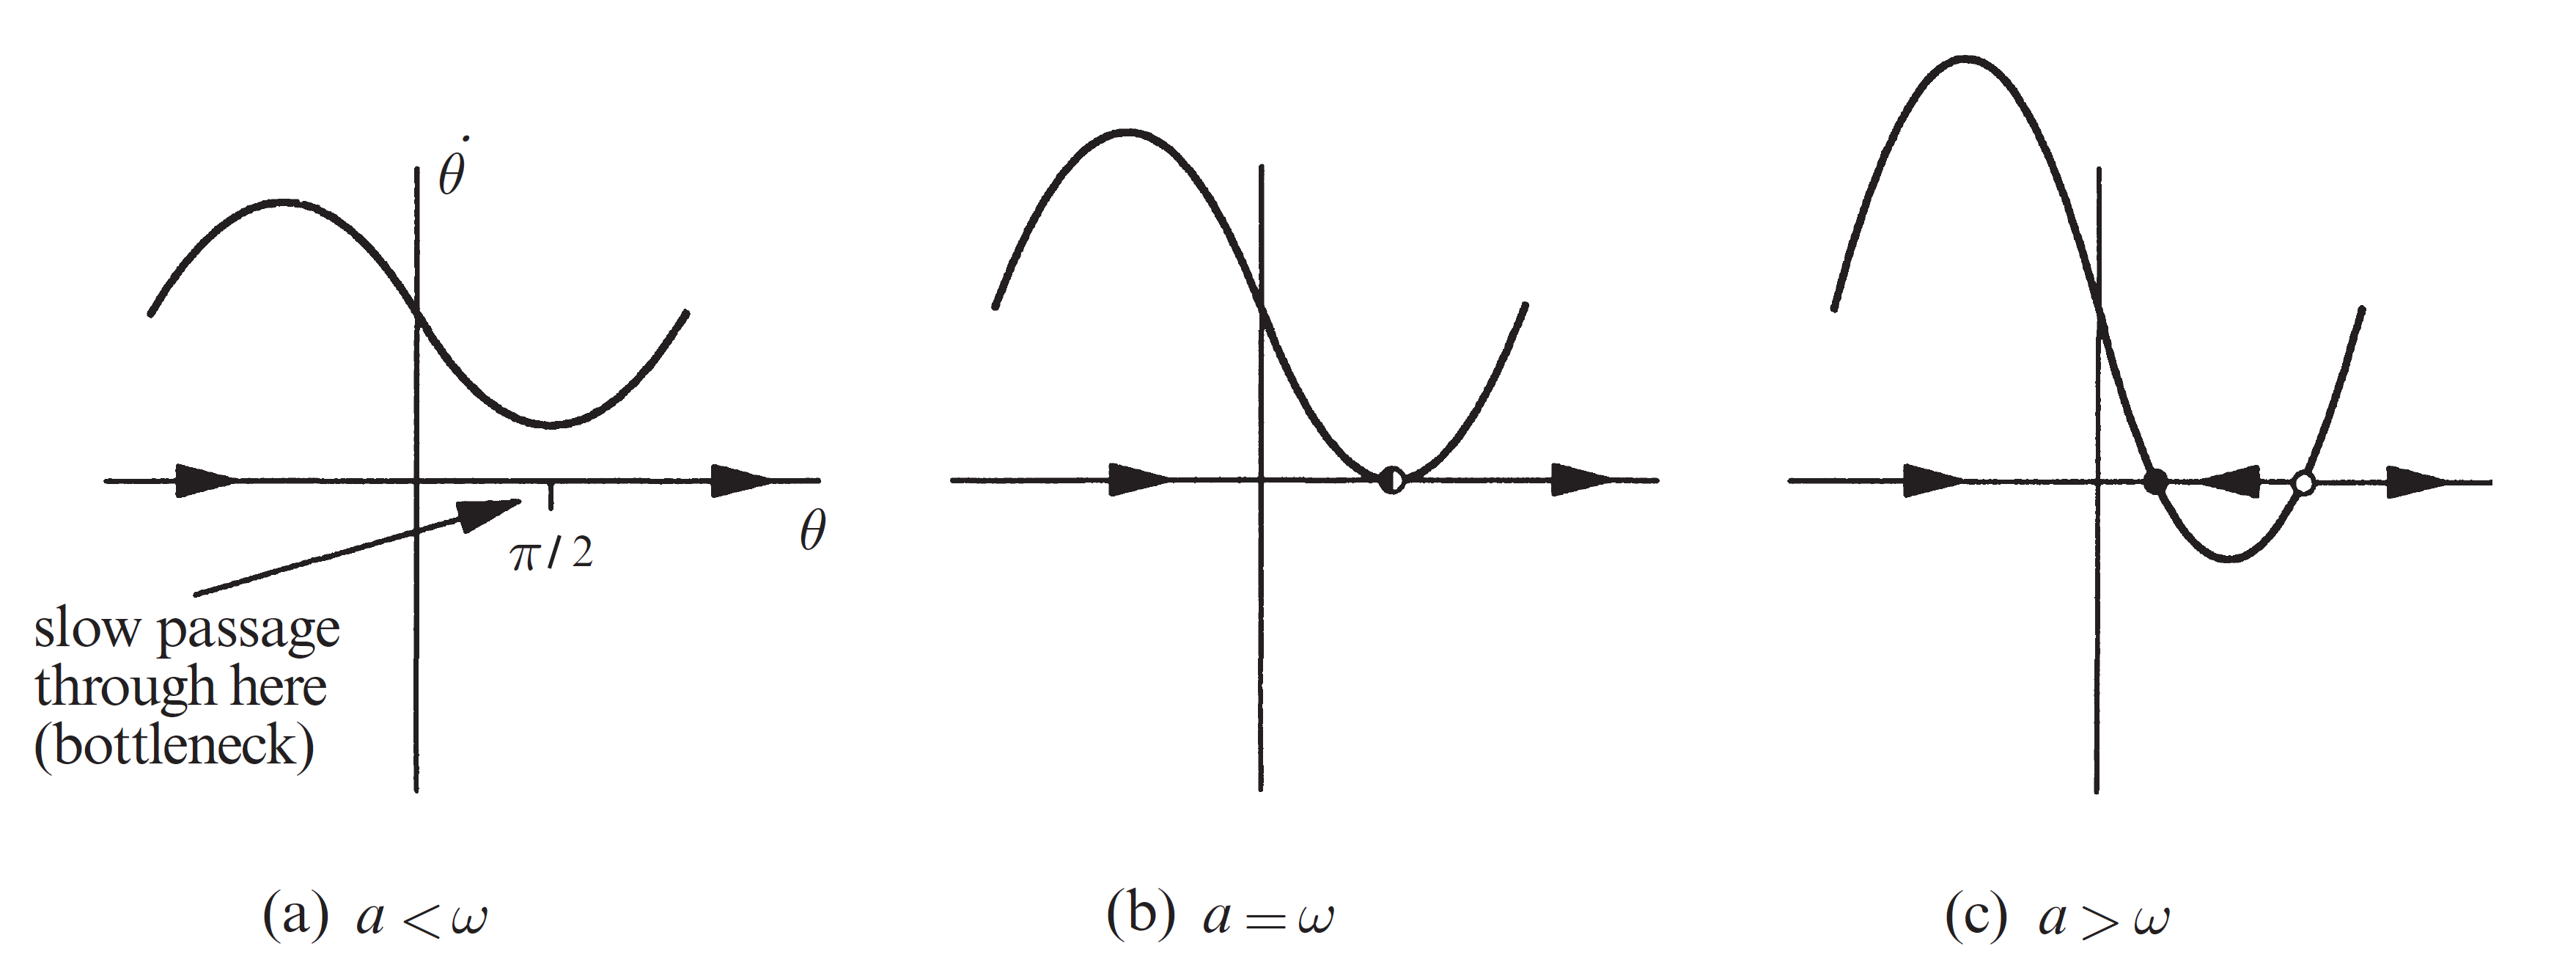
\includegraphics[width=\linewidth]{fotc1.png}
    \caption{}
    \label{fig:fotc1}
  \end{subfigure}
  \vline
  \begin{subfigure}{0.45\linewidth}
    \centering
    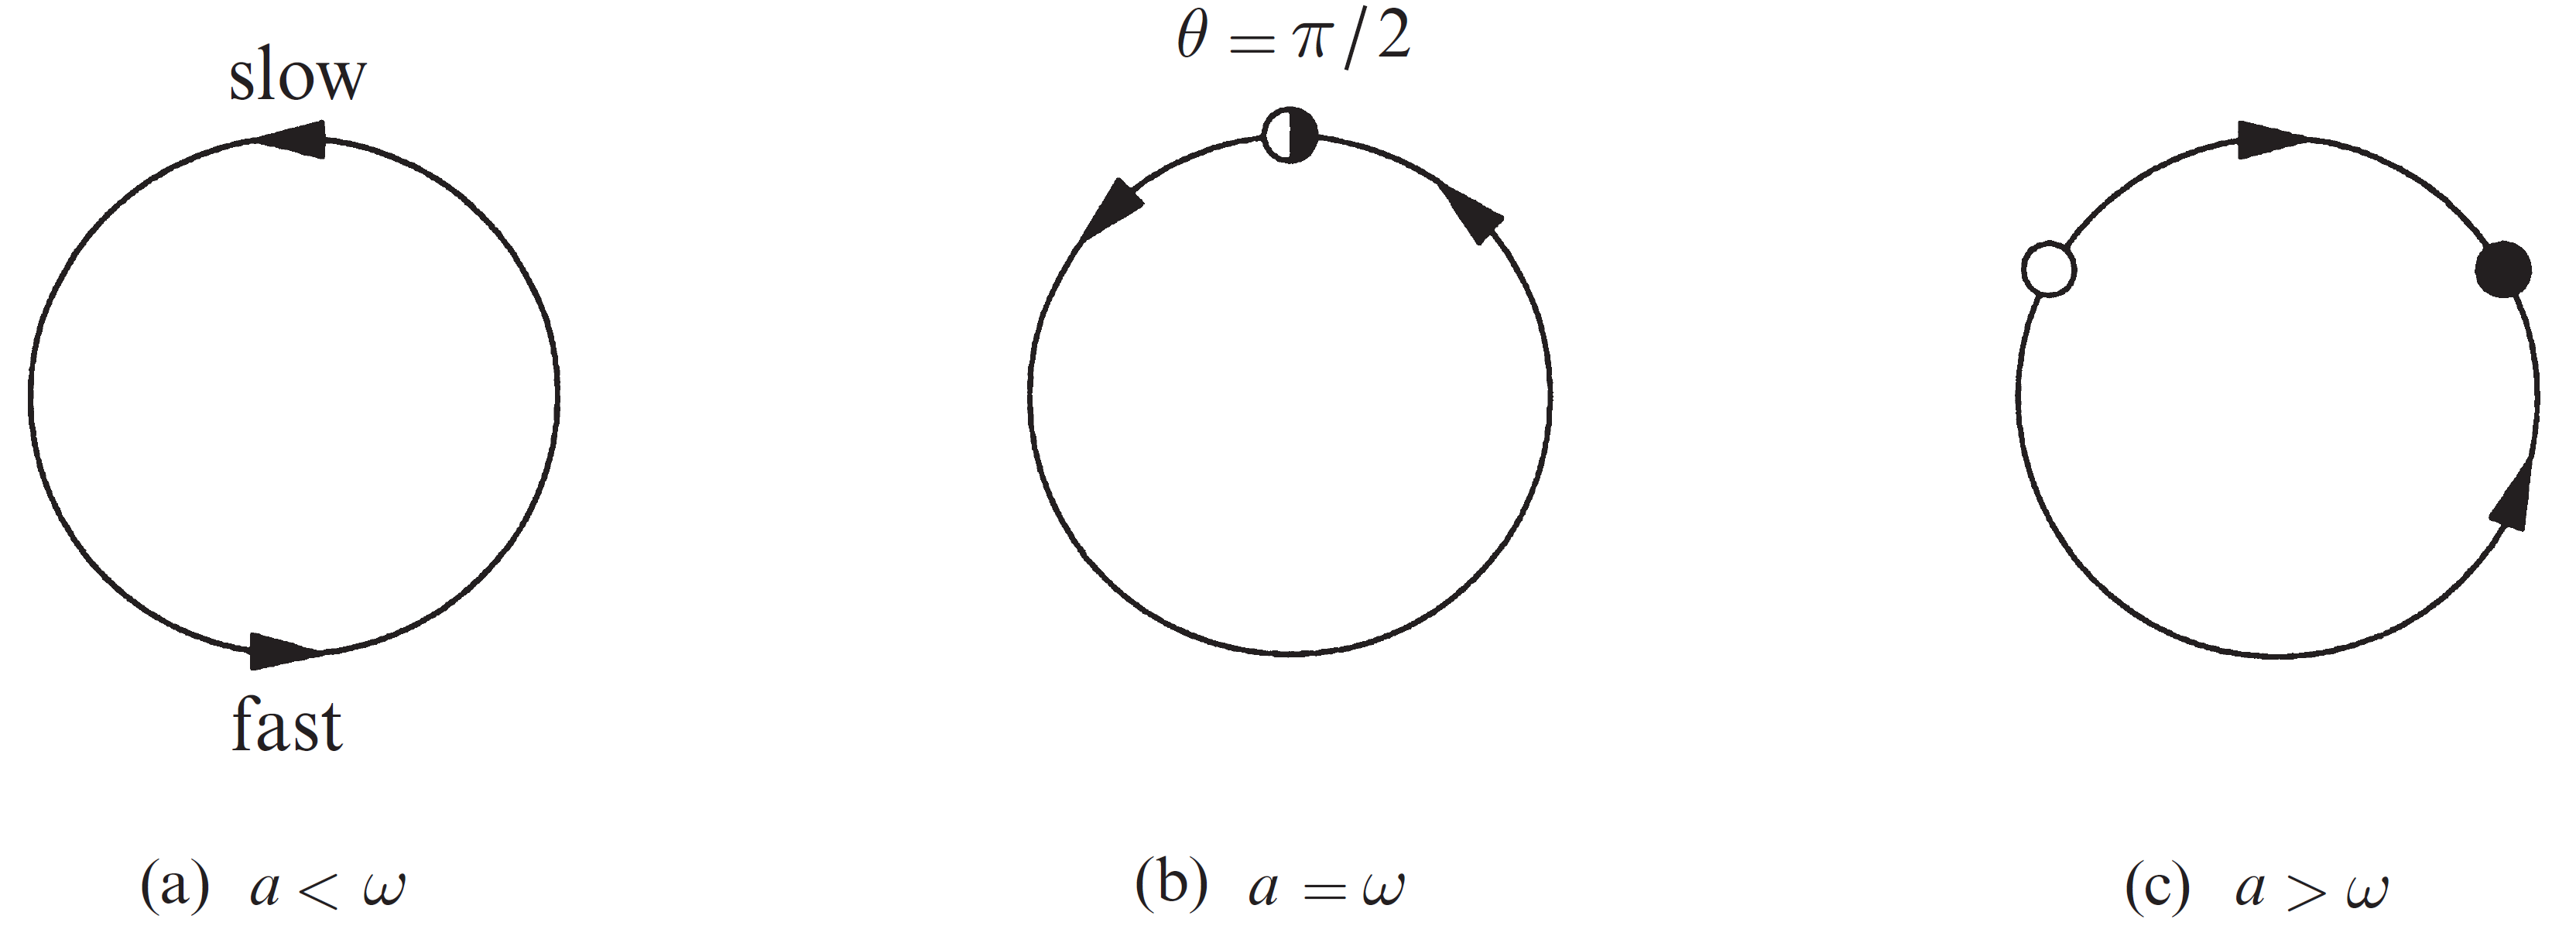
\includegraphics[width=\linewidth]{fotc2.png}
    \caption{}
    \label{fig:fotc2}
  \end{subfigure}
  \caption{}
\end{figure}
\begin{itemize}
  \item For $a<\omega$, the period of the oscillation\footnote{$$T=\int dt=\int_0^{2\pi} \frac{dt}{d\theta}d\theta=\int_0^{2\pi}\frac{d\theta}{\omega-a\sin\theta}$$} $T=\dfrac{2\pi}{\sqrt{\omega^2-a^2}}$.
  \item When $a$ is slightly less than $\omega$, the oscillation is very jerky: the phase point $\theta(t)$ takes a long time to pass through a \emph{bottleneck} near $\theta=\pi/2$, after which it zips around the rest of the circle on a much faster time scale (Figure (\ref{fig:fotc1}a)).
  \item When $a=\omega$, the system stops oscillating altogether: a half-stable fixed point has been born in a saddle-node bifurcation (See Section ({\ref{sec:snbf}})) at $\theta=\pi/2$ (Figure (\ref{fig:fotc1}b)).
  \item Finally, when $a>\omega$, the half-stable fixed point splits into a stable and unstable fixed point (Figure (\ref{fig:fotc1}c)).
  All trajectories are attracted to the stable fixed point as $t\rightarrow\infty$.
\end{itemize}
The same information can be shown by plotting the vector fields on the circle (Figure (\ref{fig:fotc2})).
\begin{comment}
\begin{figure}[H]
  \centering
  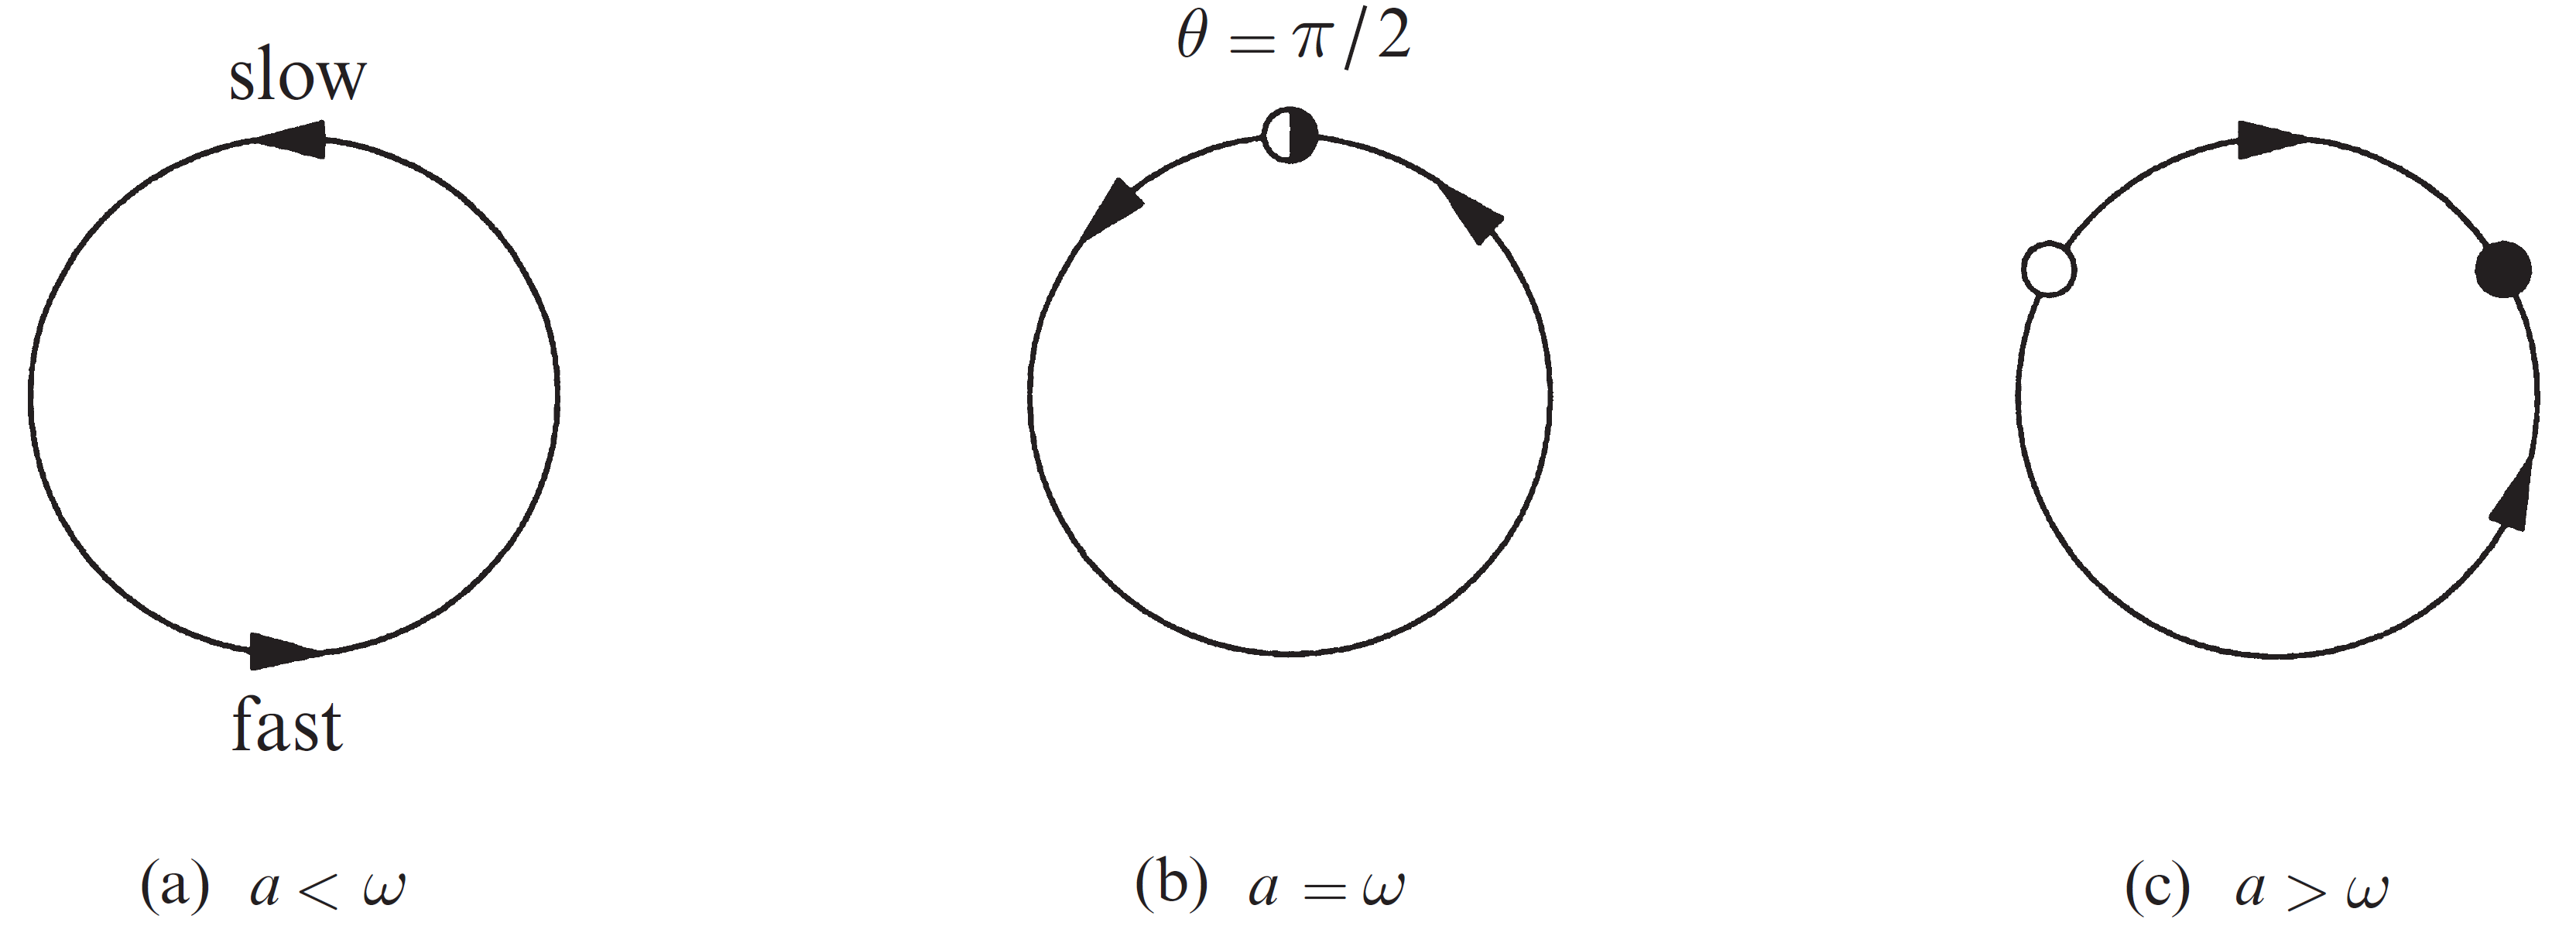
\includegraphics[width=0.5\linewidth]{fotc2.png}
  \caption{}
  \label{fig:fotc2}
\end{figure}
\end{comment}